\chapter{Literature Review}

%-------------------------------------------------------------------------------------------------------

\noindent
In this literature review we will discuss path planning with respect to courier robots, mobile agents created for the sole purpose of shipping goods. Courier robots pose a unique challenge because for the companies that use them time is literally money, so they must be able to compute these paths fast. Our main research question is how efficient are the current path planners at performing this task and how do they compare to each other. What we will analysis is the length of time it takes to produce a path, its tolerance to change, and the natural appearance of the path.\\

\noindent
The scope of this document progressively narrows, to begin with it looks at the wider application of courier robots which includes their potential benefits and economic impact. It moves on to define path planning in robotics using a grid based approach. Then three unique path planners are analysed in depth, they include \textit{Dijkstra's Algorithm} \cite{DIJKSTRA} a \textit{static} planner, \textit{D* Lite} \cite{D*LITE} a \textit{dynamic} replanner, and the main algorithm in this project \textit{Field D*} an \textit{interpolation} based replanner. Finally the findings of this literature review are discussed and presented in the conclusion.

\newpage

%-------------------------------------------------------------------------------------------------------

\section{Courier Robots}

\subsection{Field of Application}
\noindent
Until recently robots were mostly confined to industrial and military applications such as working on car assembly lines or delivering hellfire missiles to unsuspecting terrorists \cite{DRONE}. These `robots' have not changed society as visionaries like \textit{Isaac Asimov} predicted being effective in only narrow situations. Courier and delivery robots are part of an emerging branch of automation known as \textit{service robotics} \cite{SERVICE}. This new breed of robots are set to change the world that we live in today because unlike their predecessors they are becoming; (a) relatively affordable, (b) more intelligent, and (c) ubiquitous.\\

\noindent
Examples of service robots include robotic vacuum cleaners, lawn mowers, and of course self-driving cars. Every major auto manufacturer in the world is currently developing self-driving prototypes including: BMW, Mercedes, Volvo, GM, Ford, and even Google \cite{MIT}. The benefits for society span well beyond shipping goods faster and cheaper, it has the potential to save lives. Around \textit{93\%} of road traffic accidents in the US are the result of human error, driver assisted technologies can help reduce this figure \cite{ROAD}.

\subsection{Economic and Social Impact}
\noindent
No new technology comes without potential negatives, take courier robots in the transport industry which at its core involves moving items from point \textit{a} to \textit{b}, be it goods, post, or people. The incentive to adopt these new technologies is huge(!) self-driving auto-mobiles do not; tire, blink, fall a sleep, act irrationally, or demand the minimum wage. A study conducted by the University of Oxford predicted that \textit{47\%} of all jobs in the US are under threat from this new type of automation with `Cargo and Freight Agents' facing a \textit{99\%} probability that their jobs will be computerised \cite{OXFORD}. 

%-------------------------------------------------------------------------------------------------------

\section{Path Planning}

\subsection{Defining the Problem}
\noindent
Now that we have established the context for this study it is time to look at a specific task that courier robots need to accomplish. For a mobile agent to be considered useful, whether it is a vacuum cleaner, lawn mower, self-driving car, or a robotic arm, it must be able to navigate its environment. Autonomous navigation in robotics is made up of three components \cite{NEH}:

\begin{enumerate}
\item Mapping
\item Localisation
\item Path Planning
\end{enumerate}

\noindent
Mapping refers to a robots ability to discover the make-up of its environment using some form of external sensor. Localisation involves accurately establishing where a robot is in relation to its environment using a combination of internal and external sensors. Lastly there is path planning, the classic `how do I get from point \textit{a} to point \textit{b}?' problem.\\

\noindent
\textit{Path planning} is the name given to the set of steps required to reach a desired goal state from a start state \cite{HEURISTIC}. The term can be applied to a broad domain and covers everything from solving crossword puzzles to artificial intelligence, what varies is the type of states. In mobile robotics the states are typically expressed in the form of a coordinate and the task can be defined simply as `given a start state reach the goal efficiently'. By far one of the most popular ways of expressing points in relation to a robot is the \textit{Cartesian System} \cite{NEH} which is well suited to grid based path planning.

\newpage

\subsection{Representing the World as a Grid}

\noindent
There are many ways in which a robot can navigate the world around it be it using landmarks, beacons, or grids. What differs between them all is how they represent that world in memory \cite{GRIDNAV95}, what we will focus on here is grid based path planners for 2D environments. A grid based path planner uses an occupancy grid made up of individual cells that contain a probability of whether or not it is occupied.\\

\noindent
The main advantage of using a 2D grid is that it can be easily traversed as every cell is connected to eight other cells to which the robot can progress, the robot simply follows the path produced by the planner point by point (Figure: \ref{Figure: Grid.}). Updating the occupancy grid is also straight forward as the change can be mapped to the cell(s) using $x$ and $y$ coordinates. The disadvantage to this approach is memory consumption, high resolution grids require a lot of memory as each cell contains its own data used by the planner \cite{GRIDNAV95}.

\begin{figure}[htbp]

\center 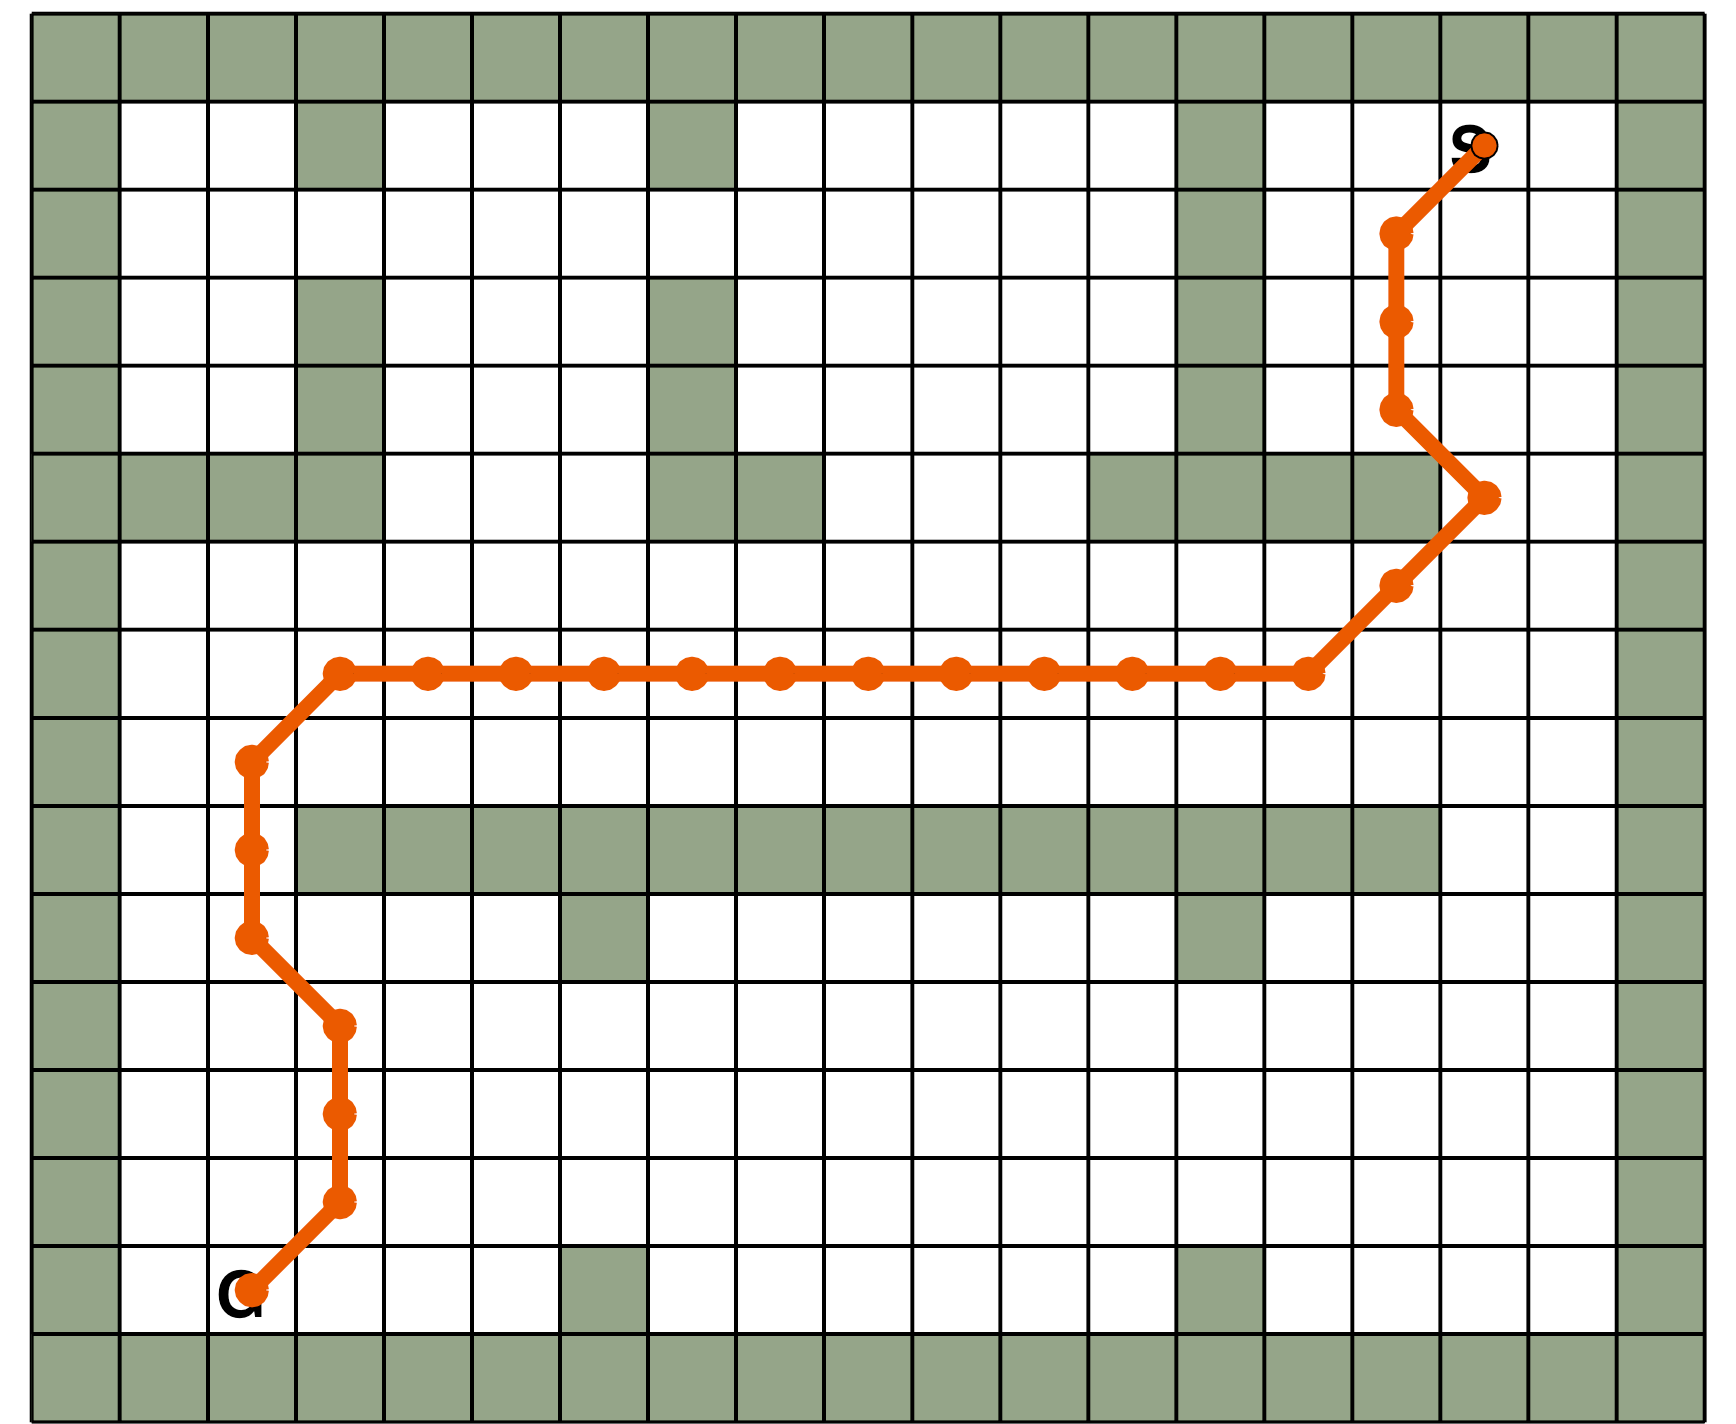
\includegraphics[width=125pt]{illustrations/grid}\\
\caption{An example of planning a path through a grid, every cell is conveniently mapped to an \textit{x} and \textit{y} position. \cite{MOTION}} 
\label{Figure: Grid.}

\end{figure}

\noindent
For example, if each cell represented $0.01m$ squared, consumed $12 bytes$ each, and the resolution of the grid was $10000cells^{2}$ it would consume $1.12GB$ of memory. That is only operating in an area that is $100m^{2}$, it is easy to see how fast a robot's resources could be exhausted and so care most be taken with this approach.

%-------------------------------------------------------------------------------------------------------

\section{Path Planning Algorithms}

\subsection{Dijkstra's Algorithm}
\noindent
In the classic path planner \textit{Dijkstra's Algorithm} \cite{DIJKSTRA} the environment (state space) is represented as a node based graph (Figure: \ref{Figure: Graph.}) defined by $\textit{G = (S, E)}$, where \textit{S} is all the possible start locations, and \textit{E} all of the traversable edges \cite{HEURISTIC}. The algorithm works by expanding outwards from the desired goal until it has computed an estimated cost for travelling from any node to the goal. It is possible to reach the desired goal from a node by iteratively traversing the edge with the lowest cost, always producing a shortest path \cite{ARNIE13}.

\begin{figure}[htbp]

\center 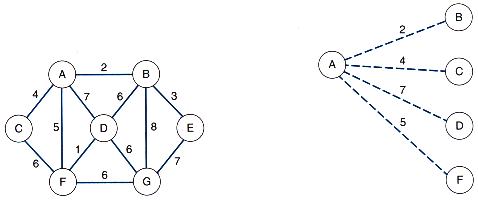
\includegraphics[width=275pt]{illustrations/graph}\\
\caption{(left) An example of a graph that has been traversed by \textit{Dijkstra's Algorithm} \cite{DIJKSTRA}. (right) All of the possible transitions from node \textit{A}, traversing the edge connected to node \textit{B} yields the lowest cost. \cite{ARNIE13}} 
\label{Figure: Graph.}

\end{figure}

\noindent
How it computes the cost for traversing an edge is dependent on the application, in the \textit{GridNav} \cite{GRIDNAV95} system (version 1.0 and 2.0) developed by Tucker Balch horizontal and vertical transitions are assigned a constant cost of \textit{1} and diagonal transitions $\sqrt{2}$. The cost of traversing an edge (cell) is the sum of all the other nodes that must be traversed to reach the goal. In his paper Balch examines path planning techniques using a go-to-goal scenario which is the basic problem that any courier robot will have to solve.\\

\noindent
Every cell in \textit{GridNav} is mapped to a node in Dijkstra's graph representation as in Figure \ref{Figure: Optimal.}(a). Each cell contains the estimated cost of travelling from that cell to the goal, occupied cells are not traversable and are assigned a high cost of \textit{500}. This approach works fine in the event that both sides of the grid are less than \textit{500} cells long. If however this were not the case it is possible that the planner would treat an occupied cell as traversable.

\begin{figure}[htbp]

\center 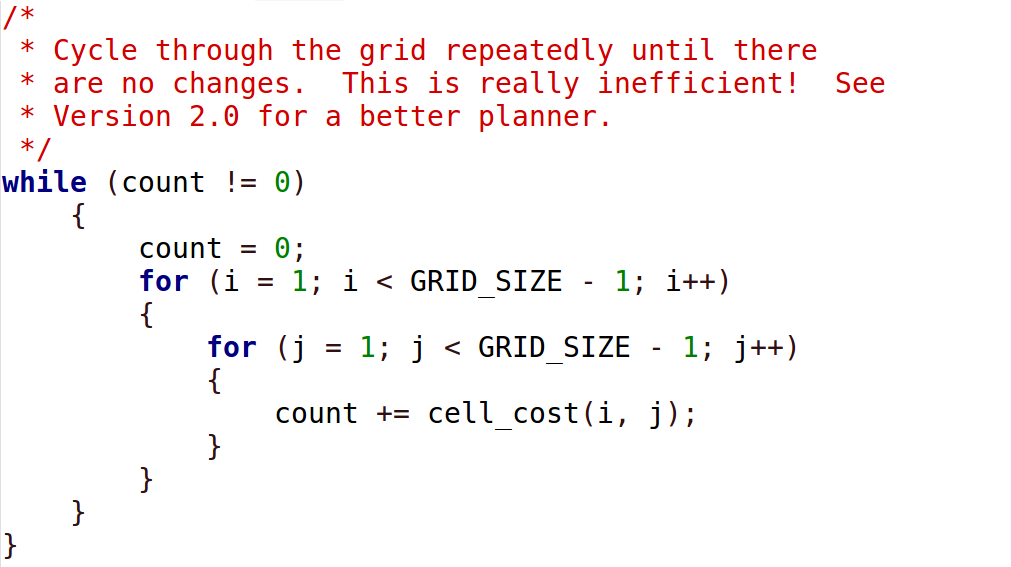
\includegraphics[width=325pt]{illustrations/version1}\\
\caption{Nested loop approach to computing the path in version \textit{1.0}. \cite{GRIDNAV95}}
\label{Figure: GridNav Version 1.0.}

\end{figure}

\noindent
While version \textit{1.0} (Figure: \ref{Figure: GridNav Version 1.0.}) is simpler to code it is \textit{extremely inefficient} \cite{GRIDNAV95} and in its worst case scenario it has an \textit{O(n)} rating of \textit{$n^{4}$}. This naive approach evaluates a cell multiple times, in the second planner a cell is only evaluated after the cost of one of its neighbours has been lowered. Balch proves this by testing the two planners on a \textit{10x10} grid, the first planner evaluated each cell \textit{10} times performing \textit{1000} evaluations compared to the enhanced planners \textit{85} evaluations. Running the planners against any grid proves that the second planner is always \textit{N} times faster, where \textit{N} is the longest side of the grid \cite{GRIDNAV95}.\\ 

\noindent
The main advantage of \textit{Dijkstra's Algorithm} is its simplicity, Balch covers the algorithm in a novel way using real code and sample results, making it a lot easier to understand compared to a purely algorithmic approach. However \textit{Dijkstra's Algorithm} is far from perfect and comes with a significant drawback, when a change is detected every edge cost must be recalculated \cite{GRIDNAV95}. These recalculations can be very expensive  when using high resolution grids \cite{HEURISTIC} as the planner considers every cell and not just the ones the robot is likely to travel through. 

\newpage

\subsection{D* Lite}
\noindent
As we have just previously discussed the task of having to solve every search from scratch, as with \textit{Dijkstra's Algorithm}, is far from practical in the dynamic environment that a courier robot is likely to operate in. Our primary concern is that such operations can be extremely computationally expensive \cite{HEURISTIC}, taking several seconds to complete when performed in large state spaces \cite{D*LITE}. A better solution would be to take the previous path and repair it based on the changes to the graph, this is the approach taken by \textit{incremental replanning algorithms}.\\

\noindent
Two of the most widely used replanning algorithms are \textit{D*} \cite{D*} and \textit{D* Lite} \cite{D*LITE} (both derived from \textit{A*} \cite{A*}) which have been tested on real robots with great success (Figure: \ref{Figure: D* Robots.}). The \textit{A*} algorithm is considered a \textit{static} planner meaning as with \textit{Dijkstra's Algorithm} it too must recompute every cost when a change to the graph occurs. When building a path \textit{A*} uses heuristics to focus the search between the start and goal positions \cite{A*} which generally results in far less evaluations than \textit{Dijkstra's Algorithm}, making \textit{A*} more efficient. \textit{D*} and \textit{D* Lite} inherit these heuristics and are not only more efficient when searching but also \textit{dynamic} as they do not need to solve every search from scratch.\\

\begin{figure}[htbp]

\center 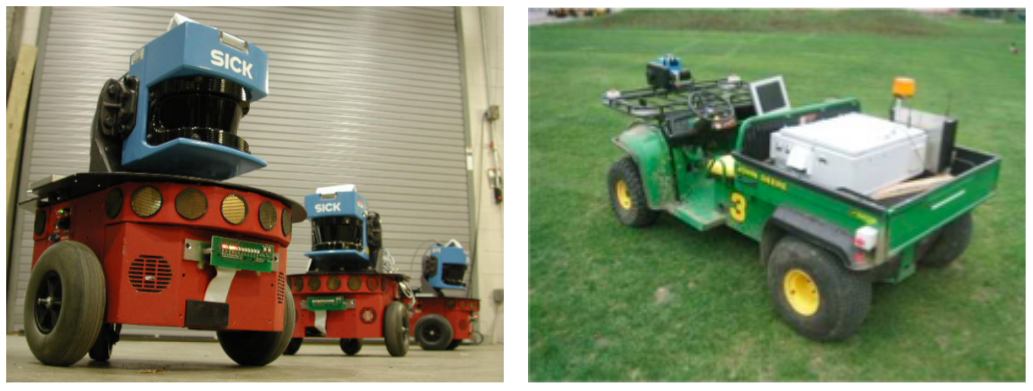
\includegraphics[width=250pt]{illustrations/example_robots}\\
\caption{\textit{D*} and \textit{D* Lite} have both been tested on real robot platforms with great success including the Pioneers (left) and the E-Gator (right). \cite{HEURISTIC}}
\label{Figure: D* Robots.}

\end{figure}

\noindent
Since \textit{D* Lite} is both eaiser to understand and more efficient \cite{HEURISTIC}\cite{D*LITE} than \textit{D*} we will focus on it alone. \textit{D* Lite} uses the same underlying graph representation, blocked cells are not traversable and no cost is associated with them, unknown cells are considered traversable until proven otherwise. Initially \textit{D* Lite} computes the cost grid just like in \cite{GRIDNAV95} however it stores additional state information such as the status of all the successors of a cell and estimated goal distances. Using this it can quickly repair broken paths by evaluating only those cells that have been affected by the update, see Figure \ref{Figure: D* Lite Path.} for an example.\\

\noindent
\textit{D* Lite's} authors provided a number of experimental results with their work which compared the algorithms performance to \textit{A*} and \textit{D*}. These experiments were carried out in simulated environments and included a number of common operations such as the total number of vertex expansions and heap percolates \cite{D*LITE}. Their findings showed that \textit{D* Lite} outperformed the other two algorithms in all of the tests and in its worst case scenario it is at least as efficient as \textit{D*}. These results are significant as \textit{D* Lite} achieves this using less operations, making it easier to understand and extend \cite{HEURISTIC}.

\begin{figure}[htbp]

\center 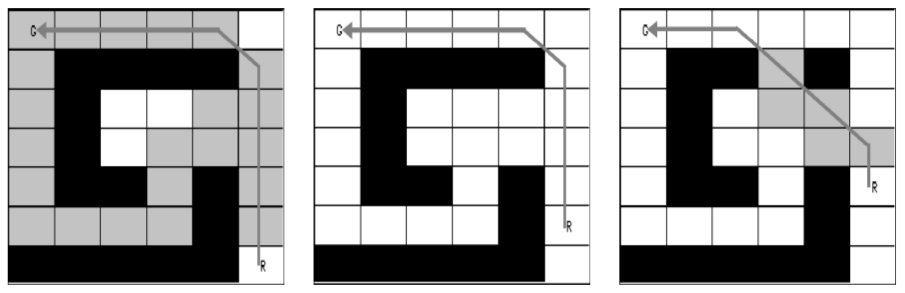
\includegraphics[width=275pt]{illustrations/d*_lite_path}\\
\caption{(left) The initial planning step evaluates the state of \textit{22} cells. (center) Path produced from the initial plan. (right) When a shorter route is discovered only \textit{5} cells need be evaluated.  \cite{HEURISTIC}}
\label{Figure: D* Lite Path.}

\end{figure}

\noindent
It is the speed and efficiency of the replanning stage that gives \textit{D* Lite} an edge over its alternatives. It is both more efficient than \textit{A*} and \textit{D*}, and removing the need to recalculate the entire cost grid makes it considerably more efficient than \textit{Dijkstra's Algorithm}. While this algorithm is a suitable path planner for a courier robot there is a significant disadvantage related to how it represents the world around it which we will discuss next.

\newpage

\subsection{Field D*}
\noindent
All of the planners that we have covered up until this point tailor an underlying graph structure to a grid, the paths they produce are therefore constrained by this limited representation. In these planners the center of every cell is connected to eight other cell centers as seen in Figure \ref{Figure: Optimal.}(a) and the robot must pass through one of these to progress. This limits the robot's headings to increments of $\dfrac{\pi}{4}$, these `optimal' paths are often unnatural, suboptimal, and difficult to traverse in practice \cite{FIELD}.\\ 

\noindent
Consider a robot in an obstacle free environment that is facing its goal, path planning is carried out using \textit{D* Lite}, and the robot's heading is $\dfrac{\pi}{8}$. The shortest path to the goal is a straight line but with planners like \textit{D* Lite} the path contains several complicated manoeuvres, this costs a delivery robot time and energy. In Figure \ref{Figure: Shortest Path.} the robot's heading is initially $\dfrac{\pi}{8}$, \textit{D* Lite} would shift this by $\dfrac{\pi}{8}$, follow $\overrightarrow{e_{1}}$, turn $\dfrac{\pi}{4}$, and continue along $\overrightarrow{e_{2}}$ to reach \textit{g}. If \textit{D* Lite} was not limited to headings of $\dfrac{\pi}{4}$ the same could be achieved simply by passing through $\overrightarrow{e_{0}}$.

\begin{figure}[htbp]

\center 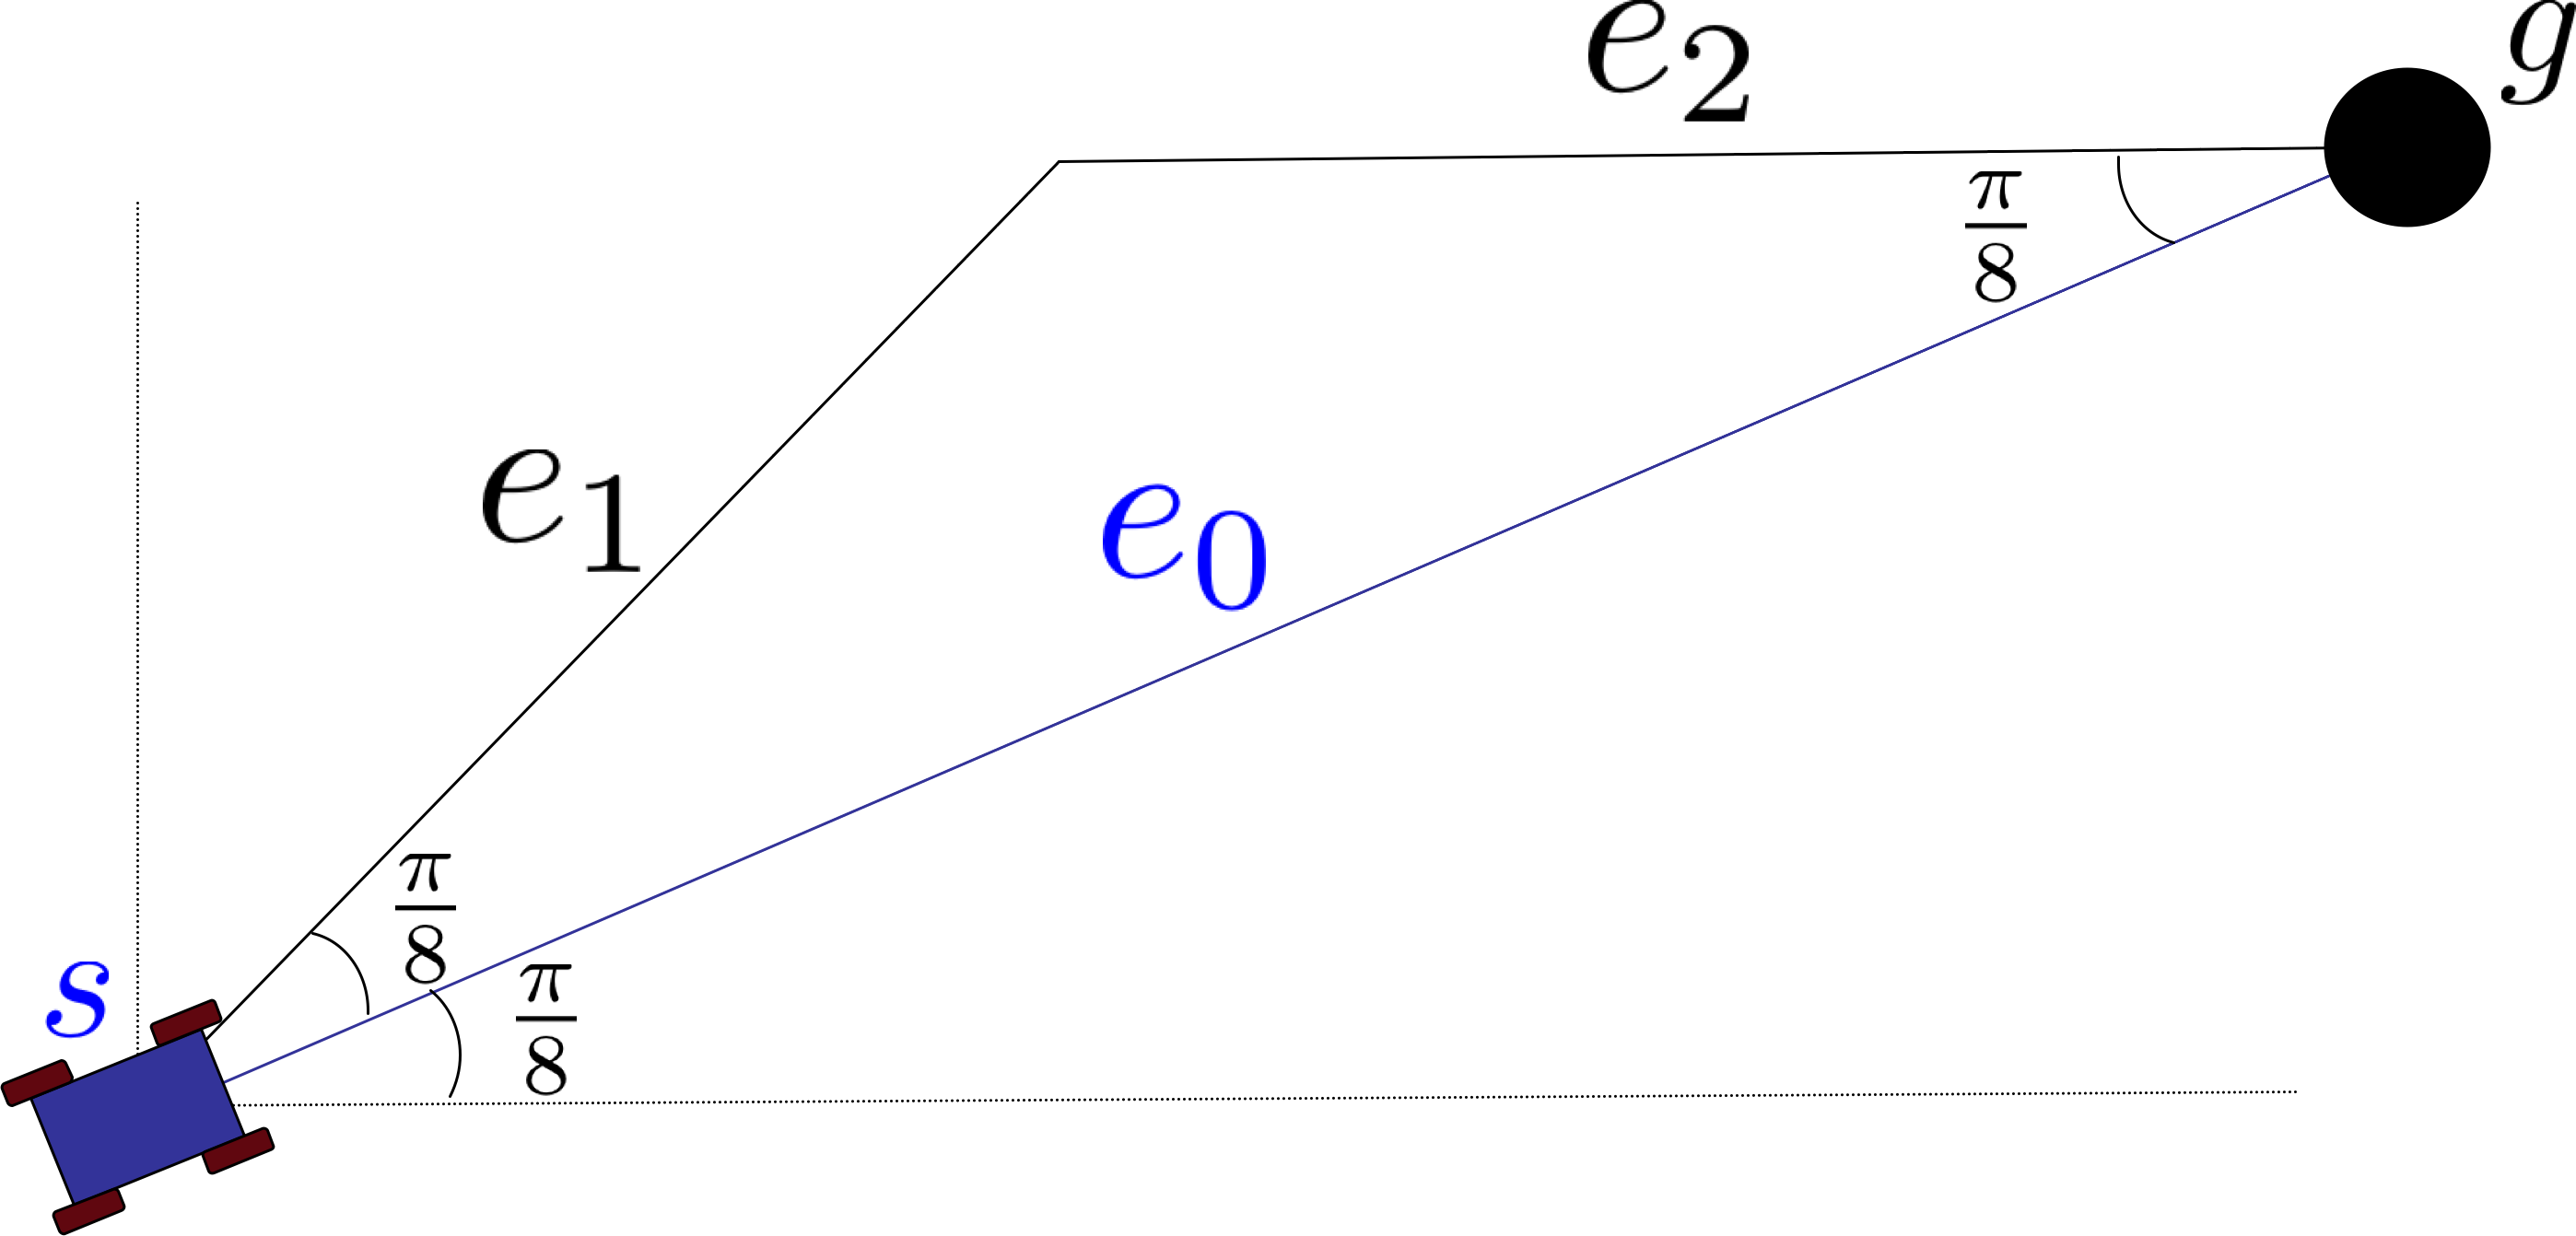
\includegraphics[width=400pt]{illustrations/shortest_path}\\
\caption{The shortest path here is along the vertex $e_{0}$, but with planners such as \textit{D* Lite} the robot must correct its heading and pass through $e_{1}e_{2}$. \cite{FIELD}} 
\label{Figure: Shortest Path.}

\end{figure}

\newpage

\noindent
Since courier robots typically function in human environments it is desirable that they choose what to a human would be the most natural path from point \textit{a} to \textit{b}. \textit{Field D*} \cite{FIELD2} is an algorithm capable of producing these `near natural' paths as it does not constrain a robots heading to increments of $\dfrac{\pi}{4}$. To achieve this \textit{Field D*} shifts the cell node from the center to the corners of each grid cell, resulting in the nodes \textit{s} to $s_{8}$ (Figure \ref{Figure: Optimal.}(b)). From these nodes we can establish the following edges $\lbrace \overrightarrow{s_{1}s_{2}}, \overrightarrow{s_{2}s_{3}}, \overrightarrow{s_{3}s_{4}}, \overrightarrow{s_{4}s_{5}}, \overrightarrow{s_{5}s_{6}}, \overrightarrow{s_{6}s_{7}}, \overrightarrow{s_{7}s_{8}}, \overrightarrow{s_{8}s_{1}} \rbrace$ \cite{FIELD}, and so the `optimal' path must intersect one of these edges (Figure \ref{Figure: Optimal.}(c)).

\begin{figure}[htbp]

\center 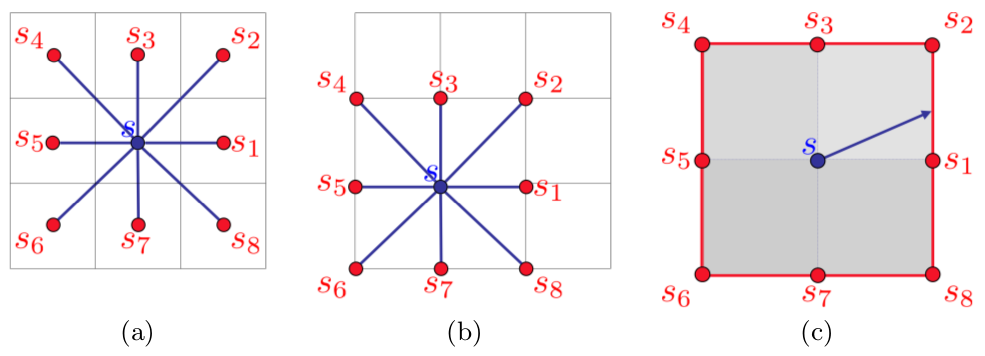
\includegraphics[width=350pt]{illustrations/nodes}\\
\caption{(a) The grid as a standard path planner represents it with the nodes appearing in the center. (b) How \textit{Field D*} treats cells with the nodes shifted to the corners. (c) The optimal path will intersect one of the defined edges at any heading. \cite{FIELD}} 
\label{Figure: Optimal.}

\end{figure}

\noindent
It was important that we first discussed \textit{D* Lite} in Subsection 1.3.2 because in its basic unoptimised form \textit{Field D*} is simply an extension of \textit{D* Lite}. At its core the algorithm uses \textit{linear interpolation} when calculating the cost of traversing a node and \textit{trigonometric maths} when computing the heading. In all of the previously mentioned path planners the cost of travelling to the goal from a node is computed as:\ 

\begin{center}
\begin{large}
$g(s) = min_{s'\in nbrs(s)}$ $(c(s,s') + g(s'))$
\end{large}
\end{center}

\noindent
Where $nbrs(s)$ is all of the nodes neighbouring $s$, $c(s,s')$ is the cost of traversing $s$ to $s'$, and $g(s')$ is the path cost of node $s'$ \cite{FIELD2}. As Stentz and Ferguson explain this formula only allows for straight-line trajectories from $s$ to a neighbouring node, which constrains the robot to headings of increment $\dfrac{\pi}{4}$. In \textit{Field D*} this assumption is relaxed to allow for headings that intersect a grid cell anywhere along its boundary at the point $g(s_{b})$ using an approximation. In Figure \ref{Figure: Optimal.}(c) we see that the optimal path intersects the edge $\overrightarrow{s_{1}s_{2}}$, to compute the cost of node $s$, Stentz and Ferguson use the following formula:

\begin{center}
\begin{large}
$g(s_{b}) = yg(s_{2}) + (1 - y)g(s_{1})$
\end{large}
\end{center}

\noindent
The path cost of $g(s_{b})$ is therefore the linear combination of the costs of $s_{1}$ and $s_{2}$, where $y$ is the distance from $s_{b}$ to $s_{1}$ \cite{FIELD2}. Stentz and Ferguson go on to discuss the theory behind \textit{Field D*} in great detail to such an extent that it cannot be fully covered here.

\begin{figure}[htbp]

\center 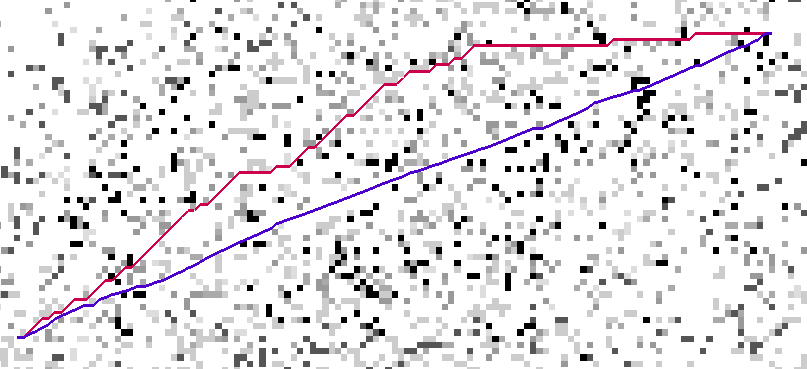
\includegraphics[width=350pt]{illustrations/field_d_path}\\
\caption{A comparison of the paths produce by \textit{Field D*} (blue) and D* Lite (red). \cite{FIELD}} 
\label{Figure: Field D Path.}

\end{figure}  

\noindent
The real value of \textit{Field D*} is the length of the paths it produces when compared to other algorithms, in Figure \ref{Figure: Field D Path.} the path produced by \textit{Field D*} is around \textit{8\%} shorter than \textit{D* Lite's} result. It is also considerably smoother and contains less turning making it easier to traverse in practice. Another advantage is that it is capable of producing these smooth paths in very low resolution grids, saving on memory \cite{FIELD}.

%-------------------------------------------------------------------------------------------------------

\newpage

\section{Discussion}
During the course of this literature review we discussed courier robots in considerable detail, covering everything from their general application to specific algorithms that enable them to operate in complex environments. As we have seen path planning is an important component in courier robots because at its simplest delivering goods is all about being able to get from \textit{a} to \textit{b}. To achieve this we need to ensure that a courier robot can reuse the knowledge it has gained during its operation and apply it efficiently to the task at hand.\\

\noindent
We looked at three different algorithms that can be used to produce a path through a grid, each of which have their individual strengths and weaknesses. Take \textit{Dijkstra's Algorithm} a \textit{greedy} algorithm that requires that the entire cost grid be recomputed every time a change occurs. Clearly this \textit{static} planner is unsuited to the fast paced environments like the one \textit{Kiva} operates in \cite{AZK12}, though it is easy to implement. Then came \textit{D* Lite} the \textit{dynamic} replanner that is capable of dealing with broken paths or identifying short cuts efficiently, yet it too is limited not by its speed but by the headings it can deal with. Finally we arrived at \textit{Field D*}.\\

\noindent
What is really promising about \textit{Field D*} is the scope of its application, NASA's Spirit, Opportunity, and Curiosity rovers that landed on Mars all used a flavour of \textit{Field D*} \cite{MARS}. If \textit{Field D*} is capable of dealing with path planning on another planet it can then surely be applied to planning efficient routes for courier robots. As with any approach there are shortcomings to \textit{Field D*} as some of the heading changes are still unnecessary \cite{THETA*}, but the paths are still considerably smoother than before. So as a result of undertaking this literature review this project has benefited from a clearly established context and a newly narrowed the focus, which will hopefully contribute towards its successful outcome.

%-------------------------------------------------------------------------------------------------------

\newpage


